% !TEX root = ../main.tex
\documentclass[../main.tex]{subfiles}

\begin{document}
\section{GitHub Actions}

Github Actions were used to run the tests and check the code formatting on every push to the main branch of the repository and on every pull request.
The configuration file for the GitHub Actions is located in the \texttt{.github/workflows} directory of the repository.
It consists of two jobs: \texttt{test} and \texttt{lint}.

The pipelines were run on self-hosted runners as it is much faster than using the GitHub-hosted runners.
Running pipelines on self-hosted runners also does not contribute to the monthly minutes limit of the GitHub runners.

\begin{figure}[H]
  \centering
  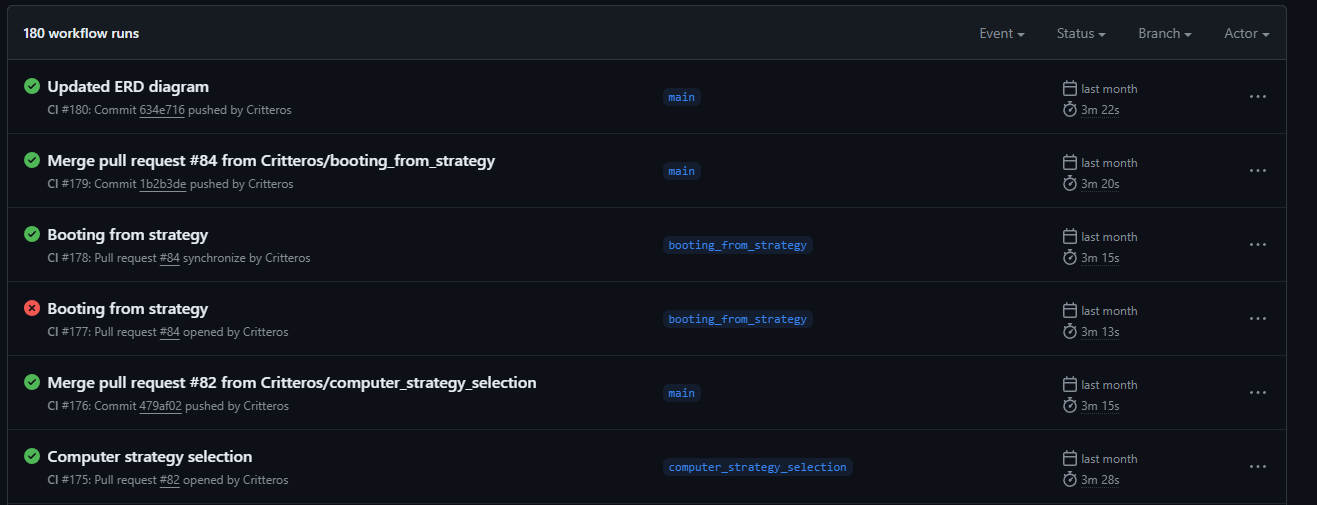
\includegraphics[width=\textwidth]{development/actions.png}
  \caption{GitHub Actions pipelines}
\end{figure}

\section{Issues and pull requests}

Github issues were used to describe the features that were to be implemented. The issues were also used to track bugs and other problems with the application.
Pull request were used to implement individual features and bug fixes.

\begin{figure}[H]
  \centering
  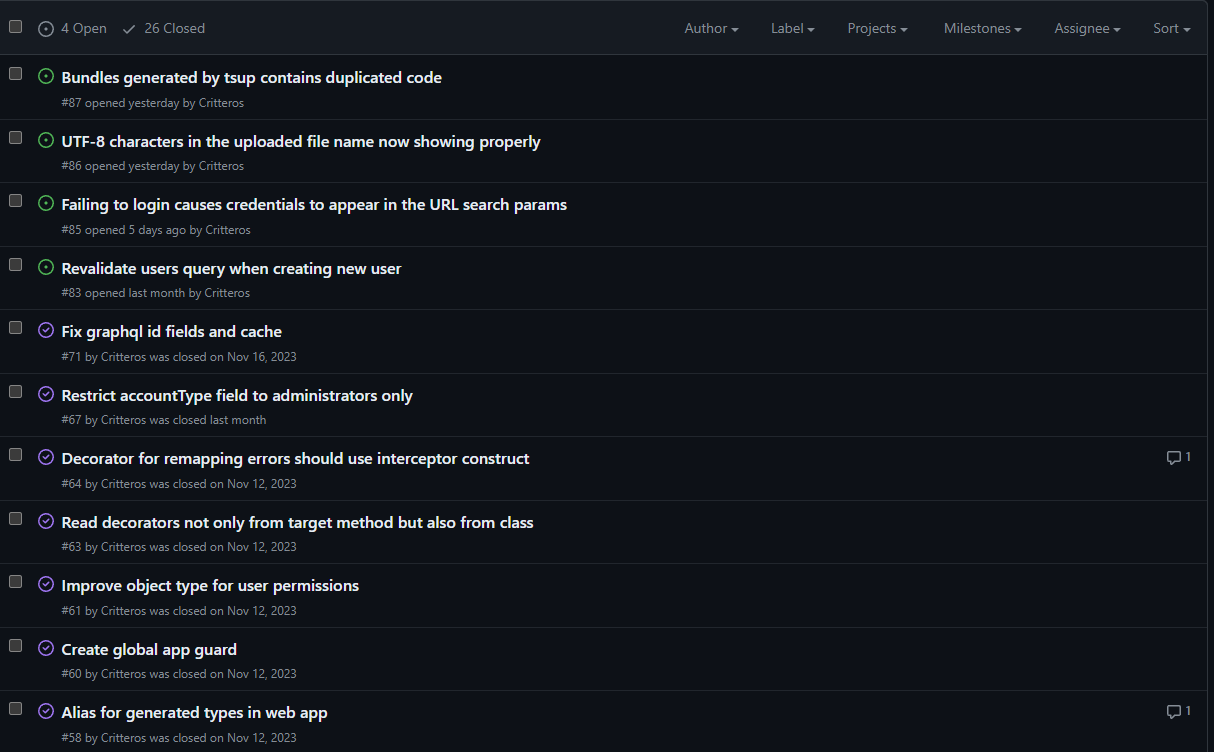
\includegraphics[width=\textwidth]{development/issues.png}
  \caption{GitHub Issues}
\end{figure}

\begin{figure}[H]
  \centering
  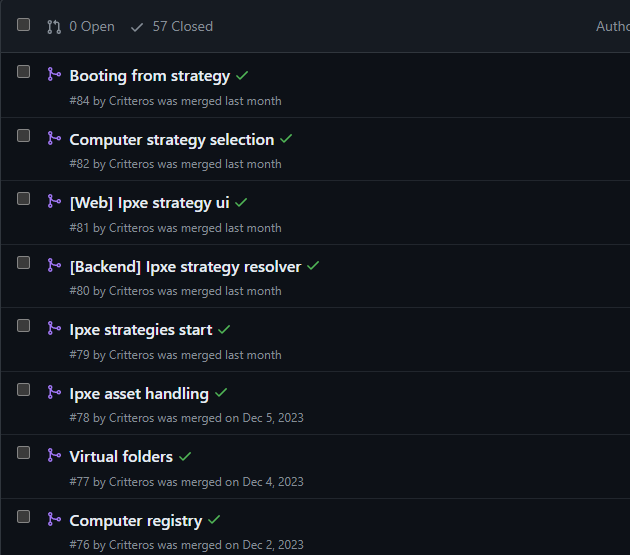
\includegraphics[width=\textwidth]{development/pull-requests.png}
  \caption{GitHub Issues}
\end{figure}

This workflow allowed to track the progress of the project and to easily see what features were implemented and what features are still to be implemented.
Any recently identified bugs were logged as issues in the repository for future resolution.


\end{document}